\section{Installation}
The installation of the UNiNOx start by configuring the Morfeas System, by adding a Morfeas\_NOX\_if component to on of the CAN-ifs.
This done from the Morfeas "System Configuration" WEB utility.
The CAN-if that will used by the Morfeas\_NOX\_if need to be free from other components and been set to 250kbps.
The baudrate setup done from the "Network Configuration" WEB utility.

After the configuration of the Morfeas system and the baudrate of the used CAN-if, the hardware can be connected at the specified CAN-if.
The figure \ref{fig:NOX_conn} show a connection diagram example.

\begin{figure}[h]
\centering
	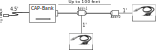
\includegraphics[width=5in,angle=0]{../art/Morfeas_web_if/connection_diagram.png}
	\caption{Morfeas UNiNOx Connection Diagram}
	\label{fig:NOX_conn}
\end{figure}

The connection after the dedicated CAN-if is followed by the "CAP-Bank",
which is a power supply that regulate the supply line for the UNiNOx(s).
The "CAP-Bank" have integrated a 4.5 feet cable that terminate on a 4pin LEMO connector, which connect to that CAN-if.
On the other side of the "CAP-Bank" there is a female 4 pin LEMO connector that accepting extension cables with connect it to
the UNiNOx adapters. The UNiNOx adapters are two kinds, one with one female side and one with two.
The adapter with one female connector is self terminated and wired the UNiNOx to address:0.
The adapter with two connectors (Tee type) wiring the UNiNOx to address:1, and in case that used alone need to be terminated with $120\Omega$.
The maximum allowed distance between the "CAP-Bank" and the last UNiNOx adapter is 100 feet. 
\textbf{ONLY} two UNiNOx can be exist at the same chain.

\begin{figure}[h]
\centering
	\includegraphics[width=5in,angle=0]{../art/Morfeas_web_if/UniNOx_adapters.png}
	\caption{"CAP-Bank" and UNiNOx adapters}
\end{figure}
